\section{Air System Distribution Terminals }\label{air-system-distribution-terminals}

\subsection{Constant Volume Single Duct Uncontrolled Air Terminal}\label{constant-volume-single-duct-uncontrolled-air-terminal}

The input object AirTerminal:SingleDuct:Uncontrolled provides a method for directly connecting a central air system to a thermal zone.~ Central system air is usually supplied to a zone through a terminal unit such as a single duct VAV reheat box.~ Sometimes, however, it is desirable to supply central system air directly to a zone without any zone level control or tempering.~ An example would be Furnace or Central DX equipment.~ AirTerminal:SingleDuct:Uncontrolled is the input object for a component used to pass supply air directly into a zone without any thermostatic control.~ This unit allows the program to know what zone this branch of the air system is attached to and a place to input the maximum air flow rate.~ It is typically used with an AirLoopHVAC running as a constant-volume, variable-temperature system.

The AirTerminal:SingleDuct:Uncontrolled object creates the capability of supplying central system air directly to a zone and only contains the zone inlet node.~ This node is both the zone inlet node and the outlet node of the AirLoopHVAC:ZoneSplitter.~ It can be thought of as a balancing damper in the duct branch going to the zone.~ This inlet flow can be controlled by an availability schedule.~ This can be thought of as a seasonal shut off of the balancing damper.

For the AirTerminal:SingleDuct:Uncontrolled objects to work correctly, it is important in any systems including them for the sum of the maximum zone air flow rates to be equal to the maximum central system flow rate.~ The zone maximum flow rates are specified in the direct air inputs.~ The central air system flow rate is specified in the AirLoopHVAC input and also in the air loop branch and central fan inputs.

\subsection{Constant Volume Single Duct Reheat Air Terminal}\label{constant-volume-single-duct-reheat-air-terminal}

The input object AirTerminal:SingleDuct:ConstantVolume:Reheat provides a model for single duct constant volume systems with reheat that satisfy the cooling load in a zone by changing the inlet air temperature with a reheat coil. The supply air temperature must be low enough to meet the cooling load in the zone having the greatest load. For zones with a smaller cooling load, a reheat coil is used to raise the temperature of the zone inlet air.

This object can be configured with a water, steam, electric or gas reheat coil. Operation is basically the same with all coil types. The coil is controlled to raise the zone supply air temperature (i.e., the Unit Air Outlet Node temperature) to match the zone load.~ If the coil is undersized, the zone setpoint temperature will not be maintained.

\begin{figure}[hbtp] % fig 153
\centering
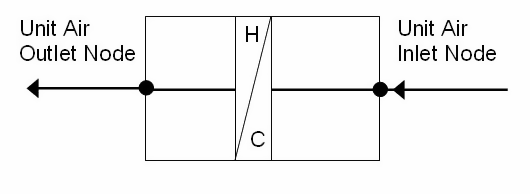
\includegraphics[width=0.9\textwidth, height=0.9\textheight, keepaspectratio=true]{media/image2788.png}
\caption{Schematic of AirTerminal:SingleDuct:ConstantVolume:Reheat Unit \protect \label{fig:schematic-of-airterminal-singleduct1}}
\end{figure}


\subsection{Constant Volume Single Duct No Reheat Air Terminal}\label{constant-volume-single-duct-no-reheat-air-terminal}

The input object AirTerminal:SingleDuct:ConstantVolume:NoReheat is used to pass conditioned or treated central supply air directly into a zone without any reheat. This terminal air equipment allows to supply central system air directly to a zone without any zone level control or tempering. The supply air temperature is controlled by the central system to meet the load in a controlled zone. This object is configured for use with a constant volume central air system, unitary system or furnace and variable supply air temperature. 

This unit allows the program to know what zone this branch of the air system is attached to, and has input fields for availability schedule, air inlet and outlet nodes, an input field for the maximum air flow rate, and other two optional input fields. The air inlet node should be the same as one of the \emph{AirLoopHVAC:ZoneSplitter} or \emph{AirLoopHVAC:SupplyPlenum} component outlet nodes. The air outlet node name should be same as zone air inlet node name and the air distribution unit air outlet node name. The last two optional input fields: \textit{Design Specification Outdoor Air Object Name}, and \textit{Per Person Ventilation Rate Mode} are used to compute the outdoor air requirement of an air terminal unit and the air terminal mass flow rate is set to the value calculated using these two input fields. 

\begin{figure}[hbtp] % fig 154
\centering
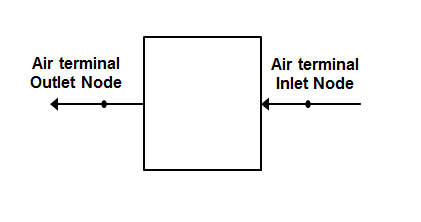
\includegraphics[width=0.9\textwidth, height=0.9\textheight, keepaspectratio=true]{media/SingleDuctConstantVolumeNoReheatAT.png}
\caption{Schematic of AirTerminal:SingleDuct:ConstantVolume:NoReheat Unit \protect \label{fig:schematic-of-airterminal-singleduct}}
\end{figure}

\subsection{Variable Air Volume Single Duct Reheat and No Reheat Air Terminals}\label{variable-air-volume-single-duct-reheat-and-no-reheat-air-terminals}

The VAV Single Duct Reheat and No Reheat terminal units (objects AirTerminal:SingleDuct:VAV:Reheat and AirTerminal:SingleDuct:VAV:NoReheat) provide models for single duct variable-air-volume (VAV) systems that control zone temperature primarily by varying the quantity of supply air rather than by varying the supply air temperature. The supply air temperature must be low enough to meet the cooling load in the zone having the greatest load when the zone terminal device is wide open. For zones with a smaller cooling load, the terminal device damper reduces the flow to match the zone setpoint.. If the lower flow limit on the terminal device is reached and the load is not matched, the inlet air temperature can be moderated if the terminal device has a reheat coil. In that case both the quantity of air and its temperature entering the zone are varied to meet the load. For air terminals using reheat coils, the maximum flow during reheat may be limited. Limiting the maximum flow during reheat occurs only when cooling is required (when any valid air loop cooling coil is active) and the terminal unit must reheat the air. Optional user inputs may also be used to control the amount of outdoor air entering the zone.

\begin{figure}[hbtp] % fig 155
\centering
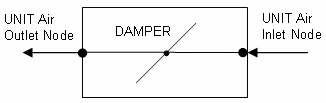
\includegraphics[width=0.9\textwidth, height=0.9\textheight, keepaspectratio=true]{media/image2789.png}
\caption{Schematic of AirTerminal:SingleDuct:VAV:NoReheat Unit \protect \label{fig:schematic-of-airterminal-singleduct-vav}}
\end{figure}

\begin{figure}[hbtp] % fig 156
\centering
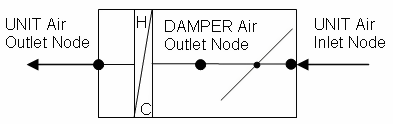
\includegraphics[width=0.9\textwidth, height=0.9\textheight, keepaspectratio=true]{media/image2790.png}
\caption{Schematic of AirTerminal:SingleDuct:VAV:Reheat Unit \protect \label{fig:schematic-of-airterminal-singleduct-vav-001}}
\end{figure}

The operation of the dampers and the control are described in the section AirTerminal:SingleDuct:VAV:HeatAndCool:Reheat and \\ AirTerminal:SingleDuct:VAV:HeatAndCool:NoReheat, which follows. The exception is that the section below describes how the air flow rate is varied for both cooling and heating. For the case of AirTerminal:SingleDuct:VAV:NoReheat and AirTerminal:SingleDuct:VAV:Reheat, air flow only varies during cooling operation and the air flow rate is set at the minimum value (minimum air flow fraction) when zone heating is required.

\subsubsection{Minimum Outdoor Air Control}\label{minimum-outdoor-air-control}

The single duct air terminals may also be used to provide a minimum outdoor air quantity. When the air flow rate required to meet the zone load does not provide sufficient outdoor air, the terminal device damper will open to allow sufficient outdoor air to enter the zone. In this case, the terminal damper is controlled based on the air loop's outdoor air fraction. The outdoor air may be specified as a fixed value per person, per floor area, or per zone. The minimum outdoor air may also be specified as air changes per hour. In addition, these values may be added together to provide a combined minimum outdoor air flow rate or the maximum of each of these values may be used. An outdoor air fraction schedule may also be used to modify the calculation for the minimum amount of outdoor air throughout the simulation (Ref. DesignSpecification:OutdoorAir).

\subsection{Variable Air Volume Heating and Cooling Single Duct Reheat and NoReheat Air Terminal}\label{variable-air-volume-heating-and-cooling-single-duct-reheat-and-noreheat-air-terminal}

\subsubsection{Overview}\label{overview-001}

The VAV Heating and Cooling Single Duct Reheat and No Reheat terminal units (objects AirTerminal:SingleDuct:VAV:HeatAndCool:Reheat and Air\-Ter\-minal:\-Single\-Duct:\-VAV:\-Heat\-And\-Cool:\-No\-Re\-heat provide models for variable-air-volume (VAV) terminal units are widely used in commercial and industrial applications. The VAV terminal units contain actuated dampers that vary the amount of central system air supplied to a zone. These terminal units may also contain a heating coil to trim the supply air temperature when overcooling is possible. The heating coil may also serve as the primary air heating source when the central system contains cooling-only equipment.

The VAV terminal units described here are used primarily with central air handling equipment with cooling and heating capability. The terminal unit dampers modulate in \textbf{both} cooling and heating mode to maintain the zone setpoint temperature(s). The central air handling equipment may be either variable air volume or constant volume where a bypass duct is used to shunt excess system air flow back to the inlet of the central air handler as terminal unit dampers modulate to satisfy the zone thermostat (i.e., AirLoopHVAC:UnitaryHeatCool:VAVChangeoverBypass).

\subsubsection{Model Description}\label{model-description-000}

The no reheat version of the single duct VAV heat and cool terminal unit contains a single virtual damper assembly and requires minimal inputs. The reheat version contains both a virtual damper assembly and an air reheat coil. Multiple reheat coil types are available:

1)~~~Coil:Heating:Water

2)~~~Coil:Heating:Electric

3)~~~Coil:Heating:Fuel

4)~~~Coil:Heating:Steam

Both units are simulated to provide an air flow rate sufficient to satisfy the thermostat request. The air flow rate is a function of the terminal unit's inlet air temperature and the load sensed by the thermostat. The output of the models are simply the damper position required to satisfy the zone's thermal load. Other information regarding terminal unit performance may be viewed using node report variables and heating coil report variables.

\begin{figure}[hbtp] % fig 157
\centering
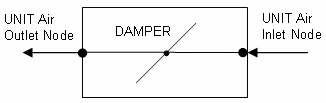
\includegraphics[width=0.9\textwidth, height=0.9\textheight, keepaspectratio=true]{media/image2791.png}
\caption{Schematic of AirTerminal:SingleDuct:VAV:HeatAndCool:NoReheat Unit \protect \label{fig:schematic-of-airterminal-singleduct-vav-002}}
\end{figure}

\begin{figure}[hbtp] % fig 158
\centering
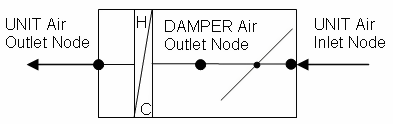
\includegraphics[width=0.9\textwidth, height=0.9\textheight, keepaspectratio=true]{media/image2792.png}
\caption{Schematic of AirTerminal:SingleDuct:VAV:HeatAndCool:Reheat Unit \protect \label{fig:schematic-of-airterminal-singleduct-vav-003}}
\end{figure}

\subsubsection{Terminal Unit Inputs}\label{terminal-unit-inputs}

Both terminal unit types share several common input fields. A unique terminal unit name must be entered. A system availability schedule is also defined to allow operational control of the terminal unit. The user must then connect the unit to the air distribution system by defining the unit inlet and outlet node names. Design air flow rates are then specified: maximum total air flow rate (autosizable) and minimum air flow fraction.

The reheat version of this terminal unit requires additional information. The name and type of reheat coil and the damper air outlet node name (same as reheat coil inlet node name). Maximum and minimum water flow rates are entered when a water or steam heating coil is used, as well as a control node name for actuating water-side flow rates and a convergence tolerance for iteration control.

\subsubsection{Simulation and Control}\label{simulation-and-control}

The simulation begins by determining the air mass flow rate required to satisfy the heating/cooling demand.

\begin{equation}
C{p_{zone}} = PsyCpAirFnWTdb\left( {{\omega_{zone}},{T_{zone}}} \right)
\end{equation}

\begin{equation}
C{p_{inlet}} = PsyCpAirFnWTdb\left( {{\omega_{inlet}},{T_{inlet}}} \right)
\end{equation}

\begin{equation}
DeltaCpT = \left( {C{p_{inlet}}} \right)\left( {{T_{inlet}}} \right) - \left( {C{p_{zone}}} \right)\left( {{T_{zone}}} \right)
\end{equation}

\begin{equation}
  \dot{m} = \min \PB{ \dot{m}_{max}, \max \PB{ \dot{m}_{max}\times MinAirFlowFrac,\frac{\dot{Q}_{zone}}{DeltaCpT} } }
\end{equation}

where:

\(C{p_{zone}}\) = Specific heat of zone air, J/kg-K

\(C{p_{inlet}}\) = Specific heat of terminal unit inlet air, J/kg-K

\({\omega_{zone}}\) = Zone air humidity ratio, kg/kg

\({T_{zone}}\) = Zone air dry-bulb temperature, °C

\({\omega_{inlet}}\) = Terminal unit inlet air humidity ratio, kg/kg

\({T_{inlet}}\) = Terminal unit inlet air dry-bulb temperature, °C

\({\dot Q_{zone}}\) = Zone load, W (positive values denote heating, negative values denote cooling)

\(\dot m\) = Terminal unit air mass flow rate, kg/s

\(PsyCpAirFnWTdb\) = Psychrometric function calculating air specific heat given air humidity ratio and dry-bulb temperature

\(MinAirFlowFrac\) = User-specified zone minimum air flow fraction

\({\dot m_{max}}\) = Terminal unit maximum air mass flow rate, kg/s.

The outdoor air input fields, if entered, are then used to adjust the terminal unit air mass flow rate to ensure the correct amount of outdoor air enters the zone (within the constraints of the terminal unit maximum and minimum flow rate inputs). The amount of outdoor air is calculated per the outdoor air requirements and is adjusted by the fraction of outdoor air entering the air loop outdoor air system.

\begin{equation}
\dot m = \max \left( \dot m, \frac{\dot m_{OA}}{OAFrac} \right)
\end{equation}

where:

\(\dot m_{OA}\) = zone outdoor air flow rate, kg/s

\(OAFrac\) = fraction of outdoor air entering the air loop outside air system.

If the terminal unit is in reheat mode (i.e., the central air loop cooling coil is active, the supply air was overcooled, and the zone thermostat is requesting heating) the maximum air flow rate allowed during reheat mode is adjusted as necessary.

\begin{equation}
\mathop m\limits^\cdot  \, = \,MIN\left( {\mathop m\limits^\cdot  ,\,{{\mathop m\limits^\cdot  }_{reheat}}} \right)
\end{equation}

where \(\dot m_{reheat}\) = maximum air mass flow rate during reheat, kg/s

The damper position is then calculated as:

\begin{equation}
FRAC_{damper} = \frac{\dot m}{\dot m_{max}}
\end{equation}

and the amount of outdoor air entering the zone is:

\begin{equation}
\dot V_{OA} = \dot m (OAFrac)
\end{equation}

where:

\(FRAC_{damper}\) = Output variable `Zone Air Terminal VAV Damper Position', fraction of maximum flow

\(\dot V_{OA}\) = Output variable ``Zone Air Terminal Outdoor Air Volume Flow Rate'' entering the zone, m\(^3\)/s.

Simulation of the reheat coil occurs next when applicable. The heating demand required to maintain the thermostat heating setpoint temperature and the heating capacity of air flowing through the terminal unit are used to determine the amount of reheat required.

\begin{equation}
{\dot Q_{reheat}} = {\dot Q_{heatSP}} + \dot m C_{p,zone}(T_{inlet}-T_{zone})
\end{equation}

where:

\({\dot Q_{reheat}}\) = Reheat coil load, W (positive values denote heating)

\({\dot Q_{heatSP}}\) = Load to heating setpoint temperature, W (positive values denote heating).

\subsubsection{References}\label{references-001}

No specific references.

\subsection{Constant Volume Single Duct Four Pipe Induction Air Terminal}\label{constant-volume-single-duct-four-pipe-induction-air-terminal}

The four pipe induction terminal unit (object name: \\ AirTerminal:SingleDuct:ConstantVolume:FourPipeInduction) is a hybrid air-hydronic unit that supplies both centrally conditioned air and local hydronic heating/cooling to a zone. Centrally conditioned air is supplied to the terminal unit at high pressure and constant flow. The central (primary) air is discharged into the terminal unit through a nozzle, inducing a fixed flow of zone (secondary) through a hydronic heating/cooling coil. The primary and secondary air streams mix and are discharged to the zone. Hot or cold water flow through the coil is varied to meet the zone heating or cooling requirement.

\subsubsection{Model}\label{model}

The four pipe induction terminal unit is modeled as a compound component consisting of three sub-components: a hot water coil, a chilled water coil and an air mixer. In terms of EnergyPlus objects these are \emph{Coil:Heating:Water}, \emph{Coil:Cooling:Water}, and \emph{AirLoopHVAC:ZoneSplitter}.~ The terminal unit is a forward model: its inputs are defined by the state of its inlets: namely its 2 air streams -- primary and secondary; and its two water inlets -- hot and cold. The outputs of the model are the conditions of the outlet air stream: flow rate, temperature and humidity ratio. The terminal unit data and simulation are encapsulated in the module \emph{HVACSingleDuctInduc}.

\subsubsection{Inputs and Data}\label{inputs-and-data}

The user describes the terminal unit by inputting the name and type of the heating and cooling coils and the name of the zone mixer. The user must also specify the connectivity of the component by naming the inlet air and water nodes and the air outlet node. Finally maximum and fixed flow rates need to be specified (although these can be autosized): maximum and minimum hot and cold water volumetric flow rates and the total air volumetric flow rate (sum of primary and secondary flow rates). The relative convergence tolerances for the hot and cold water flow rates also need to be input (or allowed to default). Finally the induction ratio needs to be specified: this~ is defined as the ratio of the secondary air flow rate to the primary air flow rate. The relationship between the flow rates is:

\begin{equation}
{\dot m_{air,tot}} = {\dot m_{air,pri}} + {\dot m_{air,\sec }}
\end{equation}

\begin{equation}
{\dot m_{air,sec}} = {R_{induc}}\cdot {\dot m_{air,pri}}
\end{equation}

so:

\begin{equation}
{\dot m_{air,pri}} = {\dot m_{air,tot}}/(1 + {R_{induc}})
\end{equation}

\begin{equation}
{\dot m_{air,sec}} = {\dot m_{air,tot}}\cdot {R_{induc}}/(1 + {R_{induc}})
\end{equation}

where \emph{R\(_{induc}\)} is the user-input induction ratio.

All input data for the four pipe induction terminal units is stored in the array \emph{IndUnit}.

\subsubsection{Calculation}\label{calculation}

Given the needed inputs, the output is calculated in subroutine \emph{CalcFourPipeIndUnit}. The temperature, humidity ratio and flow rate of the primary and secondary air streams are taken from the inlet air nodes. The inlet hot and chilled water flow rates are passed in as parameters -- temperatures are taken from the inlet water nodes. Then:

The hot water coil is simulated (Call \emph{SimulateWaterCoilComponents);}

The chilled water coil is simulated (Call \emph{SimulateWaterCoilComponents});

The two air streams are mixed (Call \emph{SimAirMixer}).

Finally the load met by the terminal unit is calculated and passed back to the calling routine:

\begin{equation}
{\dot Q_{out}} = {\dot m_{tot}}\cdot {c_{p,air}}\cdot ({T_{air,out}} - {T_{air,zone}})
\end{equation}

Note that data is never explicitly passed between the sub-components. This is all handled automatically by the node connections and the data stored on the nodes.

\subsubsection{Simulation and Control}\label{simulation-and-control-1}

From the result of the zone simulation, we have the heating/cooling demand on the terminal unit \({\dot Q_{z,req}}\). For a given hot and cold water flow \emph{CalcFourPipeIndUnit} will give us the terminal unit heating/cooling output. We need to vary the hot or cold water flow to make the unit output match the demand. To do this we need to numerically invert \emph{CalcFourPipeIndUnit}: given the output, we want one of the inputs -- the hot or cold water flow. The numerical inversion is carried out by calling subroutine \emph{SolveRegulaFalsi}. This is a general utility routine for finding the zero of a function (the \emph{residual} function) of a single independent variable. In this case, the residual function calculates \(({\dot Q_{z,req}} - {\dot Q_{out}})/{\dot Q_{z,req}}\). \emph{SolveRegulaFalsi} varies either the hot water or cold water mass flow rate to zero the residual.

Decide whether the unit is on or off. The unit is off if: a) it is scheduled off; b) the inlet air mass flow rate is zero; c) the zone thermostat is in the deadband; d) or the zone heating/cooling demand is very small.

If the unit is off, call \emph{CalcFourPipeIndUnit} with the hot and cold water flow rates set to their minimum flows and return.

If the unit is on, check whether active heating or cooling by the hydronic coils is needed. Call \emph{CalcFourPipeIndUnit} with minimum water flows to see what how much cooling (or possibly heating) the unit is doing with primary air only. The output for this case is \({\dot Q_{pri}}\).

If \({\dot Q_{z,req}} > {\dot Q_{pri}}\), we need active heating. Set the cold water flow rate to the minimum. Check that the terminal unit can meet the load by setting the hot water flow rate to the maximum and calling \emph{CalcFourPipeIndUnit}. If the output is less than the zone demand we are done -- all the outputs have been calculated. Otherwise call \emph{SolveRegulaFalsi} to obtain the hot water flow rate that will make the unit output match the zone demand. This ends the unit simulation.

If \({\dot Q_{z,req}} < {\dot Q_{pri}}\), we need active cooling. We set the hot water flow rate to the minimum. We check whether the terminal unit can supply the needed output by setting the cold water flow rate to the maximum and calling \emph{CalcFourPipeIndUnit.} If this maximum cooling output is not able to meet the zone cooling demand we are done. Otherwise call \emph{SolveRegulaFalsi} to obtain the cold water flow rate that will make the unit output match the zone demand. This ends the unit simulation.

Note that the terminal unit output is never explicitly passed to another routine. Instead the output is saved as the outlet conditions on the terminal unit outlet air node. The node data is accessed when the terminal unit output is needed elsewhere in the program (in \emph{SimZoneAirLoopEquipment} for instance).

\subsubsection{References}\label{references-1-000}

No specific references.

\subsection{Fan Powered Induction Series and Parallel Single Duct~ Reheat Air Terminal}\label{fan-powered-induction-series-and-parallel-single-duct-reheat-air-terminal}

\subsubsection{Overview}\label{overview-1-000}

The input objects AirTerminal:SingleDuct:SeriesPIU:Reheat and \\ AirTerminal:SingleDuct:ParallelPIU:Reheat provide models for fan powered induction terminal units that occur in a variety of configurations. EnergyPlus models 2 types: \emph{series} (sometimes called \emph{constant}) and \emph{parallel} (sometimes called \emph{intermittent}). The series unit provides a constant flow of air to the zone (the fan is always on at a constant flow) with a variable proportion of primary and secondary air. The parallel unit has an intermittent fan: the fan is off at maximum cooling and does not switch on until primary air flow is significantly reduced from the maximum or if reheat is required. Once on it provides a constant flow of secondary air. Both units induce air from the zone or plenum (secondary air) and mix it with centrally conditioned supply air (primary air). Both units are variable volume: the supply air flow rate is varied to match zone conditioning requirement.

\subsubsection{Model}\label{model-1}

Both types of PIU are modeled as compound components. The series unit, in sequence from its inlet, consists of an air mixer, a constant volume fan, and a heating coil. In terms of EnergyPlus objects, this is:

\begin{enumerate}
\item AirLoopHVAC:ZoneMixer
\item Fan:SystemModel or Fan:ConstantVolume
\item Coil:Heating:Water, Coil:Heating:Electric, Coil:Heating:Fuel or Coil:Heating:Steam
\end{enumerate}

The parallel unit contains a fan (in the secondary air stream, an air mixer, and a heating coil. In terms of EnergyPlus objects, this is:

\begin{enumerate}
\item Fan:SystemModel or Fan:ConstantVolume
\item AirLoopHVAC:ZoneMixer
\item Coil:Heating:Water, Coil:Heating:Electric, Coil:Heating:Fuel or Coil:Heating:Steam
\end{enumerate}

Both units are forward models: their inputs are defined by the state of their inlets: namely the air inlet and the hot water~ inlet. The outputs of the models are the conditions of the outlet air stream: flow rate, temperature and humidity ratio. The PIUs data and simulation are encapsulated in the module \emph{PoweredInductionUnits}. The main simulation routine for the units within the module are \emph{CalcSeriesPIU} and \emph{CalcParallelPIU}.

\subsubsection{Inputs and Data}\label{inputs-and-data-1}

The user describes the PIU by inputting the names of the mixer, fan and heating coil sub-components plus the type of the heating coil sub-component. The user must connect the unit to the overall HVAC systems by naming various inlet and outlet nodes: the primary air inlet node, the secondary air inlet node, the unit air outlet node, and the hot water inlet node. One internal node name is needed: the coil air inlet node (same as fan outlet mode for series, mixer outlet node for parallel). Design flow rates need to be specified (although these can be autosized): maximum total air flow rate (series), maximum primary air flow rate, minimum primary air flow fraction, maximum secondary air flow rate (parallel), fan-on flow fraction (parallel), and maximum and minimum hot water flow rates. A convergence tolerance needs to be specified for units with hot water coils. There is an on/off availability schedule that need to be set.

All input data for the powered induction terminal units is stored in the array \emph{PIU}.

\subsubsection{Calculation}\label{calculation-1}

The calculation is performed by simulating the sub-components in the order given above. Most of the code is involved with figuring out what the various flow rates should be before simulating the subcomponents. These calculations are described below.

\subsubsection{Simulation and Control}\label{simulation-and-control-2}

\emph{Series}

From the result of the zone simulation we have the heating/cooling demand on the terminal unit \({\dot Q_{tot}}\). The subroutine \emph{CalcSeriesPIU} needs to determine the flow rates that will allow the unit to meet this load. The first step is to determine the on/off state of the unit and determine the air flow rates.

\begin{itemize}
  \item
    If the unit is scheduled off, the primary and secondary flow rates are set to zero.
  \item
    If there is no primary air flow (or less than .001 kg/s), the primary air flow is set to zero and the secondary air flow is set to the constant total air flow input by the user only if there is a heating load.
  \item
    If the zone temperature is in the deadband or the zone load is less than 1 watt or the zone needs heating, the primary air flow rate is set to the minimum flow rate specified by the input and the secondary air flow rate is set to the difference between the fixed total air flow rate and the primary air flow rate.
  \item
    Otherwise, the zone needs cooling and the unit is active.
    \begin{itemize}
      \item 
        We determine the fan temperature rise: the secondary air flow is set to the max total air flow, primary air flow to zero, and the mixer and fan are simulated. The fan delta T is the difference between the temperature at the fan's outlet node and inlet node.
      \item
        We calculate the unit air outlet temperature needed to meet the zone cooling load: \({T_{out}} = {T_{z}} + {\dot Q_{z,req}}/({\dot m_{air,tot}}\cdot {c_{p,air,z}})\)
      \item
        The temperature needed at the outlet of the mixer is then: \({T_{mix}} = {T_{out}} - \Delta {T_{fan}}\)
      \item
        We can then set the primary air flow rate.
        \begin{itemize}
          \item
            If \({T_{mix}} \le {T_{in,pri}}\), then \({\dot m_{pri}} = {\dot m_{pri,max}}\)
          \item
            Else if \({T_{mix}} \ge {T_{in,pri}}\) and \({T_{mix}} \ge {T_{in,sec}}\), then \({\dot m_{pri}} = {\dot m_{pri,min}}\)
          \item
            Otherwise \({\dot m_{pri}} = {\dot m_{air,tot}}\cdot ({T_{in,sec}} - {T_{mix}})/({T_{in,sec}} - {T_{in,pri}})\), subject to the constraints that the flow rate can't be bigger than the max and min allowed.
        \end{itemize}
    \end{itemize}
\end{itemize}

The air flow rates are now determined and we can fire the air mixer (Call \emph{SimAir-Mixer}) and fan (Call \emph{SimulateFanComponents}) component simulations. Finally we simulate the heating coil:

\begin{itemize}
  \item
    for a hot water coil, if the coil is off (no flow, deadband, no load) just fire the coil simulation once (Call \emph{SimulateWaterCoilComponents}). Otherwise call \emph{ControlCompOutput}; \emph{ControlCompOutput} is a general component control routine. In this case it calls \emph{SimulateWaterCoilComponents} repeatedly while varying the hot water flow rate and minimizing

\begin{equation}
  ({c_{p,air}}\cdot {\dot m_{air,tot}}\cdot ({T_{out}} - {T_z}) - {\dot Q_{z,req}})/{\dot Q_{z,req}}
\end{equation}

to within the heating convergence tolerance.
  \item
    For gas, electric or steam coils, the required coil output is set to \({\dot Q_{coil,req}} = {\dot Q_{z,req}} - {c_{p,air}}\cdot {\dot m_{air,coil}}({T_{air,coil,in}} - {T_z})\) . Then the coil simulation is fired (Call \emph{SimulateHeatingCoilComponent} or \emph{SimulateSteamCoilCompo-nents}).
\end{itemize}

Finally the unit sensible output is calculated:

\begin{equation}
{\dot Q_{sens,out}} = {\rm{PsyHFnTdbW}}({T_{air,out}},{W_z}) - {\rm{PsyHFnTdbW(}}{T_z},{W_z})
\end{equation}

where \emph{PsyHFnTdb} is the EnergyPlus function giving enthalpy as a function of temperature and humidity ratio.

\emph{Parallel}

From the result of the zone simulation we have the heating/cooling demand on the terminal unit \({\dot Q_{tot}}\). The subroutine \emph{CalcParallelPIU} needs to determine the flow rates that will allow the unit to meet this load. The first step is to determine the on/off state of the unit and determine the air flow rates.

\begin{itemize}
  \item
    If the unit is scheduled off, the primary and secondary flow rates are set to zero.
  \item
    If there is no primary air flow (or less than .001 kg/s), the primary air flow is set to zero and the secondary air flow is set to the max secondary air flow input by the user only if there is a heating load.
  \item
    If the zone temperature is in the deadband or the zone load is less than 1 watt or the zone needs heating, the primary air flow rate is set to the minimum flow rate specified by the input. If there is a heating load or reheat is required, the secondary air flow rate is set to max secondary air flow input by the user.
  \item
    Otherwise, the zone needs cooling and the unit is active.
  \begin{itemize}
    \item
      We determine the fan temperature rise: the secondary air flow is set to the max secondary air flow, primary air flow to zero, and the fan and mixer are simulated. The fan delta T is defined as the difference between the temperature at the mixer outlet node and the fan inlet node.
    \item
      Assuming that the fan is off, we calculate the primary air flow needed to meet the cooling demand.

\begin{equation}
  {\dot m_{pri}} = {\dot Q_{z,req}}/({c_{p,air}}\cdot ({T_{in,pri}} - {T_z}))
\end{equation}

The flow rate is constrained to be between the min and max primary air flow rates. If this calculated primary flow rate is greater than the fan-on flow rate, the secondary flow rate is set to zero and we are done. Otherwise, the fan is on and we need to recalculate the primary air flow rate.

\begin{equation}
  {\dot m_{pri}} = ({\dot Q_{z,req}} - {c_{p,air}}\cdot {\dot m_{sec}}\cdot ({T_{in,sec}} + \Delta {T_{fan}} - {T_z}))/({c_{p,air}}\cdot ({T_{in,pri}} - {T_z}))
\end{equation}

The secondary flow rate is set to the user input fixed flow rate if reheat is required or if the primary air flow fraction is at or below the user-specified fan on fraction. The primary air flow rate is constrained to be between the min and max primary flow rated.
  \end{itemize}
\end{itemize}

The air flow rates are now determined and we can fire the fan (Call \emph{SimulateFanComponents}) and air mixer (Call \emph{SimAirMixer}) component simulations. Finally we simulate the heating coil:

\begin{itemize}
  \item
    For a hot water coil, if the coil is off (no flow, deadband, no load) just fire the coil simulation once (Call \emph{SimulateWaterCoilComponents}). Otherwise call \emph{ControlCompOutput}; \emph{ControlCompOutput} is a general component control routine. In this case it calls \emph{SimulateWaterCoilComponents} repeatedly while varying the hot water flow rate and minimizing

\begin{equation}
({c_{p,air}}\cdot {\dot m_{air,tot}}\cdot ({T_{out}} - {T_z}) - {\dot Q_{z,req}})/{\dot Q_{z,req}}
\end{equation}

to within the heating convergence tolerance.

  \item
    For gas, electric or steam coils, the required coil output is set to \({\dot Q_{coil,req}} = {\dot Q_{z,req}} - {c_{p,air}}\cdot {\dot m_{air,coil}}({T_{air,coil,in}} - {T_z})\) . Then the coil simulation is fired (Call \emph{SimulateHeatingCoilComponent} or \emph{SimulateSteamCoilComponents}).
\end{itemize}

Finally the unit sensible output is calculated:

\begin{equation}
{\dot Q_{sens,out}} = {\rm{PsyHFnTdbW}}({T_{air,out}},{W_z}) - {\rm{PsyHFnTdbW(}}{T_z},{W_z})
\end{equation}

where \emph{PsyHFnTdb} is the EnergyPlus function giving enthalpy as a function of temperature and humidity ratio.

\subsubsection{References}\label{references-2}

No specific references.

\subsection{Variable Air Volume Fan Powered Single Duct Air Terminal}\label{variable-air-volume-fan-powered-single-duct-air-terminal}

\subsubsection{Overview}\label{overview-2-000}

The input object AirTerminal:SingleDuct:VAV:Reheat:VariableSpeedFan provides a model for variable speed (VS) fan VAV terminal unit that is a typical VAV reheat unit with the addition of a variable-speed blower fan to assist in moving supply air from the plenum to the conditioned zone. It is typically used with under-floor air distribution systems (UFAD) where the supply air is sent at low static pressure through an under-floor supply plenum. The fan has two maximum flow rate settings: one for cooling and one for heating. The cooling maximum is usually the actual fan maximum while the heating maximum is a lesser flow rate. The fan is upstream of the heating coil (this is a blow-through unit). The heating coil can be hot-water, electric or gas. Cooling control is obtained by varying the supply air flow rate from the cooling maximum to the minimum flow rate. Heating control is established by varying both the heating coil output (or hot water flow rate for hot water coils) and the supply air flow rate. Note that for this unit the minimum supply air flow rate is the flow rate when the fan is off.

\subsubsection{Model}\label{model-2}

The VS fan VAV terminal unit is modeled as a compound component consisting of two sub-components: a fan and a heating coil. In terms of EnergyPlus objects the fan is a \emph{Fan:VariableVolume} object and the heating coil is a \emph{Coil:Heating:Water}, \emph{Coil:Heating:Electric} or a \emph{Coil:Heating:Fuel}. The terminal unit is a forward model: its inputs are defined by the state of its inlets: namely its air inlet and its hot water~ inlet, if it has a hot water coil. The outputs of the model are the conditions of the outlet air stream: flow rate, temperature and humidity ratio. The terminal unit data and simulation are encapsulated in the module \emph{SingleDuct}. The main simulation routine for the unit within the module is \emph{SimVAVVS}.

\subsubsection{Inputs and Data}\label{inputs-and-data-2}

The user describes the terminal unit by inputting the name and type of the heating coil and the name and type of the fan. The user must also specify the connectivity of the component by naming the inlet air node; the air node connecting the fan and heating coil (fan outlet, coil inlet); the unit air outlet node (same as the zone inlet node); and hot water inlet node (if any). Maximum flow rates need to be specified (although these can be autosized): maximum cooling and heating air flow rates and the maximum hot water flow rate (if there is a hot water coil). Minimum flow rates are specified by giving by giving a minimum flow fraction for the air flow and a volumetric flow rate minimum for the hot water. For the units with hot water coils the relative convergence tolerance for the hot water flow rate also needs to be input (or allowed to default).

All input data for the VS fan VAV terminal units is stored in the array \emph{Sys}.

\subsubsection{Calculation}\label{calculation-2}

Given the needed inputs, the output is calculated in subroutine \emph{CalcVAVVS}. The temperature and humidity of the supply air stream are taken from the inlet air node. The inlet air flow rate and the hot water flow rate are passed in as parameters. If the coil is electric or gas the coil heating power is passed instead of the hot water flow rate. Then

The fan is simulated (call \emph{SimulateFanComponents}). If the fan is off the fan outlet conditions are set to the inlet conditions.

The heating coil is simulated (call \emph{SimulateWaterCoilComponents} if the coil is a hot water coil; call \emph{SimulateHeatingCoilComponents} if the coil is gas or electric).

Finally the sensible load met by the terminal unit is calculated and passed back to the calling routine:

\begin{equation}
{\dot Q_{out}} = {\dot m_{air}}\cdot {c_{p,air}}\cdot ({T_{air,out}} - {T_{air,zone}})
\end{equation}

Note that data is never explicitly passed between the sub-components. This is all handled automatically by the node connections and the data stored on the nodes.

\subsubsection{Simulation and Control}\label{simulation-and-control-3}

From the result of the zone simulation we have the heating/cooling demand on the terminal unit \({\dot Q_{tot}}\). For the given inlet conditions \emph{CalcVAVVS} will give us the terminal unit heating/cooling output. We need to vary the air or hot water flow rate or the heating coil power (for gas or electric coils) to make the unit output match the demand. To do this we need to numerically invert \emph{CalcVAVVS}: given the output, we want one of the inputs -- the air or hot water flow rate or the heating coil power. The numerical inversion is carried out by calling subroutine \emph{SolveRegulaFalsi}. This is a general utility routine for finding the zero of a function (the \emph{residual} function) of a single independent variable. In this case the residual function calculates \(({\dot Q_{tot}} - {\dot Q_{out}})/{\dot Q_{tot}}\). \emph{SolveRegulaFalsi} varies either the air mass flow rate, the hot water mass flow rate or the heating coil power to zero the residual.

The unit is simulated in the following sequence.

Decide whether the unit is on or off. The unit is off if: a) it is scheduled off; b) the inlet air mass flow rate is zero; or c) the zone thermostat is in the deadband

If the unit is off, call \emph{CalcVAVVS} with flow rates set to their minimum flows and return.

If the unit is on, we need to establish the boundaries of 4 conditioning regions: a) active cooling with fan on; b) active heating with fan on; c) active heating with fan off; d) passive cooling with fan off. The heating/cooling demand will fall into one of these regions. Once the correct region is determined, we will know which model input to vary for control and thus how to invert the calculation.

To establish the boundaries of region a) we call \emph{CalcVAVVS} twice: once with the supply air flow rate set to the cooling maximum, once with the cooling air flow rate set to the minimum. In both cases the heating coil output is at the minimum and the fan is on. Call the 2 cooling outputs \({\dot Q_{cool,max,fanon}}\) and \({\dot Q_{cool,min,fanon}}\). Remembering that EnergyPlus convention is that cooling loads are negative, then if \({\dot Q_{tot}} < {\dot Q_{cool,max,fanon}}\) the terminal unit can not meet the demand. Set the air mass flow rate to the cooling maximum and call \emph{CalcVAVV} again. This concludes the simulation. If~ \({\dot Q_{cool,max,fanon}} < {\dot Q_{tot}} < {\dot Q_{cool,min,fanon}}\) the cooling demand is in the active cooling region. We hold the heating at the minimum, allow the supply air flow to vary between the cooling maximum and the minimum with the fan on, and call \emph{SolveRegulaFalsi} to obtain the supply air flow rate that will produce the unit sensible cooling output that matches the demand. This concludes the simulation.

To establish the boundaries of region b) call \emph{CalcVAVVS} twice: once with the supply air flow rate set to the heating maximum, once with the supply air flow rate set to the minimum. In both calls, if the heating coil is a hot water coil, the hot water flow rate is at the maximum. For electric and gas coils, the heating power is set to the maximum at maximum supply air flow and to zero at the minimum supply air flow. In both calls the fan is set to be on. Call the 2 heating outputs returned from the two calls to \emph{CalcVAVVS} \({\dot Q_{heat,max,fanon}}\) and \({\dot Q_{heat,min,fanon}}\). If \({\dot Q_{heat,max,fanon}} < {\dot Q_{tot}}\) the terminal unit can not meet the load. Set the air flow rate to the heating maximum and the hot water flow rate or heating coil power to the maximum and call \emph{CalcVAVVS} again. This concludes the simulation for this case. If \({\dot Q_{heat,min,fanon}} < {\dot Q_{tot}} < {\dot Q_{heat,max,fanon}}\) the heating demand is in the active heating, fan on region. For a hot water coil we call \emph{SolveRegulaFalsi} with the supply air flow rate as the input that is varied and the hot water flow rate set to the maximum. For electric and gas coils the coil power and the supply air flow rate are both varied together from their minimum to maximum in a call to \emph{SolveRegulaFalsi}.~ The call to \emph{SolveRegulaFalsi} concludes the simulation for this case.

This region only applies to terminal units with a hot water coil. To establish the boundaries of region c) the fan is set to off, the supply air flow rate is set to minimum flow and \emph{CalcVAVVS} is called twice: once with the hot water flow at maximum and once with the hot water flow at minimum. Call the two heating outputs \({\dot Q_{heat,max,fanoff}}\) and \({\dot Q_{tot}}\). If \({\dot Q_{tot}}\) is between these values, the supply air flow rate is set to its minimum, the fan is set to off, and in the call to \emph{SolveRegulaFalsi} the hot water flow rate is varied to meet the load. This concludes the simulation for this case.

If the cooling demand does not fall into cases a) -- c), the unit is assumed to be in the passive cooling state: heating is off or at the minimum, the fan is off, and the minimum supply air flow is delivered to the zone.

Note that the terminal unit output is never explicitly passed to another routine. Instead the output is saved as the outlet conditions on the terminal unit outlet air node. The node data is accessed when the terminal unit output is needed elsewhere in the program (in \emph{SimZoneAirLoopEquipment} for instance).

\subsubsection{References}\label{references-3}

No specific references.

\subsection{Four Pipe Beam Unit (AirTerminal:SingleDuct:ConstantVolume:FourPipeBeam)}\label{four-pipe-beam-unit-airterminalsingleductconstantvolumefourpipebeam}

The four pipe beam air terminal units (\emph{AirTerminal:SingleDuct:ConstantVolume:FourPipeBeam}) are ceiling-mounted, beam-type units that are provided with primary air from a central system and additional heating or cooling by inducing room air to flow over a hydronic convector. They are called \emph{four pipe} because the units are connected with two pipes for chilled water supply and return and another two pipes for hot water supply and return. A simple empirical model is used to enable using input data derived from manufacturer's catalog data.

\subsubsection{Model Description}\label{model-description-1-000}

The model assumes that the total conditioning power, \({\dot Q_{Tot}}\), is the sum of the conditioning provided by the primary air, \({\dot Q_{SA}}\), and the conditioning provided by the beam convector, \({\dot Q_{Beam}}\).

\begin{equation}
{\dot Q_{Tot}} = {{\dot Q_{SA}} + {\dot Q_{Beam}}}
\end{equation}

The primary air contribution is easily determined using:

\begin{equation}
{\dot Q_{SA}} = {{\dot m_{SA}}\cdot ({c_{p,SA}} \cdot {T_{SA}} - {c_{p,Z}} \cdot {T_{Z}})}
\end{equation}

The convector power \({\dot Q_{Beam}}\) is coupled directly to the zone air heat balance (using a source code term called \emph{NonAirSysOutput}) in a way that provides only sensible heat transfer directly to the zone air node. We therefore assume that the air terminal's convector is always dry during cooling. Many of the terms used in the performance calculations are normalized by the total length of beam in zones, \({L}\).

When the unit is operated in cooling mode, the convector power is determined using the rated normalized cooling capacity that is modified by three separate functions.

\begin{equation}
{\dot Q_{Beam, cool}} = { \dot q_{cool,rated} \cdot f_{ \Delta T_{cool,mod} }() \cdot f_{\dot m_{SA,cool,mod}}() \cdot f_{\dot m_{CW,mod}}() \cdot L }
\end{equation}

The modification factor \({f_{ \Delta T_{cool,mod} }() }\) describes how the cooling capacity is adjusted to account for the temperature difference between the zone air and the chilled water entering the convector. This empirical correction factor is intended to account for how heat transfer between the chilled water and induced room air flow depends on the temperature difference, both in terms of surface convection heat transfer and the rate of induced air flow. The function can be described using any of the single-variable curves or a lookup table. The single independent variable is the ratio between the current temperature difference, \({\Delta T_{air-CW}}\), and the temperature difference used to rate beam performance, \({\Delta T_{air-CW,rated}}\).

\begin{equation}
{f_{ \Delta T_{cool,mod} }() } = f_{ \Delta T_{cool,mod} }\left(\frac{\Delta T_{air-CW}}{\Delta T_{air-CW,rated}}\right)
\end{equation}

\begin{equation}
{\Delta T_{air-CW}} = {T_{Z}}-{T_{CW,in}}
\end{equation}

The modification factor \({f_{\dot m_{SA,cool,mod}}()}\) describes how the cooling capacity is adjusted to account for the primary air flow rate. This empirical correction factor is intended to account for how varying primary air flow rates will impact the rate that room air is induced to flow across the convector. The function can be described using any of the single-variable curves or a lookup table. The single independent variable is the ratio between the current normalized primary air flow rate, \({\dot m_{SA}}\), and the normalized flow rate used to rate beam performance, \({\dot m_{SA,rated}}\). Flow rates are normalized by dividing the total length of all the beam units in the zone. The ratio is calculated using air mass flow rates with the rated flow rate assumed to be for standard temperature and pressure at sea level so that elevation effects appear only in the numerator when the function is evaluated.

\begin{equation}
  {f_{\dot m_{SA,cool,mod}}()} = f_{\dot m_{SA,cool,mod}}\left(\frac{{\dot m_{SA}}}{{\dot m_{SA,rated}} }\right)
\end{equation}

\begin{equation}
  {\dot m_{SA}} = \frac{\dot M_{SA}}{L}
\end{equation}

\begin{equation}
  {\dot m_{SA,rated}} = {\dot v_{SA,rated}} \cdot {\rho_{air,STP}}
\end{equation}

The modification factor \(f_{\dot m_{CW,mod}}()\) describes how the cooling capacity is adjusted to account for the flow rate of chilled water through the convector. This empirical correction factor is intended to account for how varying chilled water flow rates will impact the velocity of fluid inside the pipes and the corresponding impact on the rate of surface convection heat transfer inside the convector. The function can be described using any of the single-variable curves or a lookup table. The single independent variable is the ratio between the current normalized chilled water flow rate, \({\dot m_{CW}}\), and the normalized chilled water flow rate at the rating point, \({\dot m_{CW,rated}}\).

\begin{equation}
  {f_{\dot m_{CW,mod}}()} = f_{\dot m_{CW,mod}}\left(\frac{{\dot m_{CW}}}{{\dot m_{CW,rated}}}\right)
\end{equation}

\begin{equation}
  {\dot m_{CW}} = \frac{\dot M_{CW}}{L}
\end{equation}

\begin{equation}
  {\dot m_{CW,rated}} = {\dot v_{CW,rated}} \cdot {\rho_{CW}}
\end{equation}

The model for when the unit is operated in heating mode is very similar. The convector power is determined using the rated normalized heating capacity that is modified by three separate functions.

\begin{equation}
{\dot Q_{Beam, heat}} = {\dot q_{heat,rated}}\cdot f_{ \Delta T_{heat,mod} }() \cdot f_{\dot m_{SA,heat,mod}}()\cdot f_{\dot m_{HW,mod}}() \cdot L
\end{equation}

The modification factor \(f_{ \Delta T_{heat,mod} }()\) describes how the heating capacity is adjusted to account for the temperature difference between the hot water and the zone air entering the convector. Notice that for heating the temperature difference is defined different from cooling operation so that positive difference values are the result. This empirical correction factor is intended to account for how heat transfer between the hot water and induced room air flow depends on the temperature difference, both in terms of surface convection heat transfer and induced air flow rates. The function can be described using any of the single-variable curves or a lookup table. The single independent variable is the ratio between the current temperature difference, \(\Delta T_{HW-air}\), and the temperature difference used to rate beam performance, \(\Delta T_{HW-air,rated}\).

\begin{equation}
{f_{ \Delta T_{heat,mod} }()} = f_{ \Delta T_{heat,mod} }\left(\frac{\Delta T_{HW-air}}{\Delta T_{HW-air,rated}}\right)
\end{equation}

\begin{equation}
{\Delta T_{HW-air}} = {T_{HW,in}} -{T_{Z}}
\end{equation}

The modification factor \(f_{\dot m_{SA,heat,mod}}()\) describes how the heating capacity is adjusted to account for the primary supply air flow rate. This empirical correction factor is intended to account for how varying primary air flow rates will impact the rate that room air is induced to flow across the convector. The function can be described using any of the single-variable curves or a lookup table. The single independent variable is the same ratio described above for cooling and it is assumed that the unit can be rated using the same primary air flow rate for both heating and cooling operation of the four pipe unit. Flow rates are normalized by dividing the total length of all the beam units in the zone. The ratio is calculated using air mass flow rates with the rated flow rate assumed to be for standard temperature and pressure at sea level so that elevation effects appear only in the numerator when the function is evaluated.

\begin{equation}
{f_{\dot m_{SA,heat,mod}}()} = f_{\dot m_{SA,heat,mod}}\left(\frac{{\dot m_{SA}}}{{\dot m_{SA,rated}} }\right)
\end{equation}

The modification factor \(f_{\dot m_{HW,mod}}()\) describes how the heating capacity is adjusted to account for the flow rate of hot water through the convector. This empirical correction factor is intended to account for how varying hot water flow rates will impact the velocity of fluid inside the pipes and the corresponding impact on the rate of surface convection heat transfer inside the convector. The function can be described using any of the single-variable curves or a lookup table. The single independent variable is the ratio between the current normalized hot water flow rate, \({\dot m_{HW}}\), and the normalized hot water flow rate at the rating point, \({\dot m_{HW,rated}}\).

\begin{equation}
  f_{\dot m_{HW,mod}}() = f_{\dot m_{HW,mod}}\left(\frac{{\dot m_{HW}}}{{\dot m_{HW,rated}}}\right)
\end{equation}

\begin{equation}
  {\dot m_{HW}} = \frac{\dot M_{HW}}{L}
\end{equation}

\begin{equation}
  {\dot m_{HW,rated}} = {\dot v_{HW,rated}} \cdot {\rho_{HW}}
\end{equation} 

where:

\({c_{p,SA}}\) is the specific heat of primary air entering through the air terminal unit, in J/kg-K.

\({c_{p,Z}}\) is the specific heat of zone air, in J/kg-K.

\({c_{p,CW}}\) is the specific heat of zone air, in J/kg-K.

\({f_{\dot m_{CW,mod}}()}\) is the cooling capacity modification factor function of chilled water flow rate

\({f_{ \Delta T_{cool,mod} }()}\) is the cooling capacity modification factor function of air-water temperature difference

\({f_{\dot m_{SA,cool,mod}}()}\) is the cooling capacity modification factor function of primary air flow rate

\({f_{\dot m_{HW,mod}}()}\) is the heating capacity modification factor function of hot water flow rate

\({f_{ \Delta T_{heat,mod} }()}\) is the heating capacity modification factor function of water - air temperature difference

\({f_{\dot m_{SA,heat,mod}}()}\) is the heating capacity modification factor function of primary air flow rate

\({L}\) is the total length of all beam units serving the zone, in m

\({\dot m_{CW}}\) is the mass flow rate of chilled water per meter of length, in kg/s-m

\({\dot m_{CW,rated}}\) is the mass flow rate of chilled water per meter of length at rating point, in kg/s-m

\({\dot m_{HW}}\) is the mass flow rate of hot water per meter of length, in kg/s-m

\({\dot m_{HW,rated}}\) is the mass flow rate of hot water per meter of length at rating point, in kg/s-m

\({\dot m_{SA}}\) is the mass flow rate of primary air per meter of length, in kg/s-m

\({\dot m_{SA,rated}}\) is the mass flow rate of primary air per meter of length at rating point, kg/s-m

\({\dot M_{SA}}\) is the mass flow rate of primary air entering the zone through the air terminal unit, in kg/s

\({\dot M_{CW}}\) is the mass flow rate of chilled water, kg/s

\({\dot M_{HW}}\) is the mass flow rate of hot water, kg/s

\({\dot q_{cool,rated}}\) is the rated beam cooling capacity per meter of length, in W/m.

\({\dot q_{heat,rated}}\) is the rated beam heating capacity per meter of length, in W/m.

\({\dot Q_{Beam}}\) is the conditioning power delivered to the zone by the beam convector, in W.

\({\dot Q_{SA}}\) is the conditioning power delivered to the zone by the primary air mass flow, in W.

\({\dot Q_{Tot}}\) is the total (net) conditioning power delivered to zone by the air terminal unit, in W.

\({\rho_{air,STP}}\) is the density of air at standard conditions (sea level), in kg/m\(^{3}\)

\({\rho_{air}}\) is the density of air at standard conditions adjusted for elevation), in kg/m\(^{3}\)

\({\rho_{CW}}\) is the density of chilled water, in kg/m\(^{3}\)

\({T_{SA}}\) is the dryblub temperature of the (central) primary air entering the air terminal unit, in degrees C.

\({T_{Z}}\) is the dryblub temperature of the zone air, in  \(^{\circ}\)C.

\({T_{CW,in}}\) is the temperature of chilled water entering the convector, in \(^{\circ}\)C.

\({\Delta T_{air-CW}}\) is the difference between the zone air temperature and chilled water entering the convector, \(\Delta^{\circ}\)C.

\({\Delta T_{HW-air}}\) is the difference between the water and zone air temperature entering the convector, \(\Delta^{\circ}\)C.

\({\Delta T_{air-CW,rated}}\) is the value of \({\Delta T_{air-CW}}\) at rating conditions for cooling performance, \(\Delta^{\circ}\)C.

\({\Delta T_{HW-air,rated}}\) is the value of \({\Delta T_{HW-air}}\) at rating conditions for heating performance, \(\Delta^{\circ}\)C.

\({\dot v_{SA,rated}}\) is the volume flow rate of air per meter length at rating point, in m\(^{3}\)/s-m.

\({\dot v_{CW,rated}}\) is the volume flow rate of chilled water per meter length at rating point, in m\(^{3}\)/s-m.

\({\dot v_{HW,rated}}\) is the volume flow rate of hot water per meter length at rating point, in m\(^{3}\)/s-m.

The performance capacity model described above is controlled to modulate water flow through the beam's convector using the non-linear numerical solver in EnergyPlus called Solve root solver. The predicted zone load to setpoint \({\dot Q_{Zone, Required}}\) is adjusted by \({\dot Q_{SA}}\) to determine the required beam load.

\begin{equation}
{\dot Q_{Beam, Required}} = {\dot Q_{Zone, Required}} - {\dot Q_{SA}}
\end{equation}

When \({\dot Q_{Zone, Required}}\) is negative, the beams need to provide cooling and when it is positive the beams need to provide heating. The the solver iterates the water flow rate to find a flow rate that will meet the load.

When cooling, the result for beam capacity (negative for cooling) is used to calculate the leaving temperature of the chilled water using:

\begin{equation}
{T_{CW,out}} = {T_{CW,in}} - \frac{{\dot Q_{Beam}}}{{\dot m_{CW}} \cdot {c_{p,CW}} }
\end{equation}

However, to protect from a non-physical result the leaving chilled water temperature is constrained to be no warmer than a 1.0\(^{\circ}\)C approach temperature compared to the zone air or the primary supply air. If the above result is too warm the leaving temperature and beam cooling capacity are adjusted using the following equations, and a recurring warning is issued to alert the user that there may be a problem with the cooliong performance input data.

\begin{equation}
  {T_{CW,out}} = { max( {T_{SA}} , {T_{Z}}) - 1.0 }
\end{equation}

\begin{equation}
  {\dot Q_{Beam}} = {\dot m_{CW}} \cdot {c_{p,CW}} \cdot {( {T_{CW,in}} - {T_{CW,out}})}
\end{equation}

Similarly when heating, the result for beam capacity (positive for heating) is used the calculate the leaving temperature of the hot water using,

\begin{equation}
{T_{HW,out}} = {T_{HW,in}} - \frac{{\dot Q_{Beam}}}{{\dot m_{HW}} \cdot {c_{p,HW}} }
\end{equation}

To protect from a non-physical result the leaving hot water temperature is constrained to be no cooler than a 1.0\(^{\circ}\)C approach temperature compared to the zone air or the primary supply air. If the above result is too cool the leaving temperature and beam heating capacity are adjusted using the following equations, and a recurring warning is issued to alert the user that there may be a problem with the heating performance input data.

\begin{equation}
  {T_{HW,out}} = { min( {T_{SA}} , {T_{Z}}) + 1.0 }
\end{equation}

\begin{equation}
  {\dot Q_{Beam}} = {\dot m_{CW}} \cdot {c_{p,CW}} \cdot {( {T_{HW,in}} - {T_{HW,out}}) }
\end{equation}

\subsubsection{Four Pipe Beam Sizing}\label{four-pipe-beam-sizing}

The four pipe beam model has four inputs that can be autosized:

\begin{itemize}
\item \({L}\) is the total length of all beam units serving the zone, in m
\item \({\dot V_{SA,Des}}\) is the design primary supply air volume flow rate, in m\(^{3}\)/s
\item \({\dot V_{CW,Des}}\) is the design chilled water volume flow rate, in m\(^{3}\)/s
\item \({\dot V_{HW,Des}}\) is the design hot water volume flow rate, in m\(^{3}\)/s
\end{itemize}

Because of the way the model is formulated with defaulted inputs for rated, normalized performance data, we can link the four inputs together to ensure an internally consistent set of sizes. If any one of these four inputs is not autosized (given a fixed value at input) then the other three can be computed using the normalized, rated performance data which are either input or have default values. If the total beam length is input, then the following equations are used:

\begin{equation}
  {\dot V_{SA,Des}} = {{\dot v_{SA,rated}} \cdot {L}}
\end{equation}

\begin{equation}
  {\dot V_{CW,Des}} = {{\dot v_{CW,rated}} \cdot {L}}
\end{equation} 
  
\begin{equation}
  {\dot V_{HW,Des}} = {{\dot v_{HW,rated}} \cdot {L}}
\end{equation}

If the design primary supply air flow rate is input then the beam length can be determined as follows and then water flow rates evaluated as above.

\begin{equation}
{L} = {\frac{{\dot V_{SA,Des}}}{{\dot v_{SA,rated}}}  }
\end{equation}

If the chilled water flow rate is input, then the beam length can be determined as follows and the other values evaluated as above:

\begin{equation}
{L} = {\frac{{\dot V_{CW,Des}}}{{\dot v_{CW,rated}}}  }
\end{equation}

If the hot water flow rate is input, then the beam length can be determined as follows and the other values evaluated as above:

\begin{equation}
{L} = {\frac{{\dot V_{HW,Des}}}{{\dot v_{HW,rated}}}  }
\end{equation}

When all four inputs are autosized, which is the usual case, there is no simple way to anchor the sizes and we need to use the results from the zone and system sizing calculations to determine sizes for the four pipe beam unit. The following design data from the zone and system sizing calculations are used when sizing the four pipe beam:

\({\dot V_{TU,Z,final,cool} }\) is the final zone terminal unit design volume flow rate for cooling, in m\(^{3}\)/s

\({\dot V_{TU,Z,final,heat} }\) is the final zone terminal unit design volume flow rate for heating, in m\(^{3}\)/s

\({\dot V_{Z,final,OA} }\) is the final zone design volume flow rate for minimum outdoor air mechanical ventilation, in m\(^{3}\)/s.

\({T_{SA,cool,design } }\) is the final design zone terminal unit inlet supply air temperature at cooling peak, in \(^{\circ}\)C.

\({w_{SA,cool,design } }\) is the final design zone terminal unit inlet supply air humidity ratio at cooling peak, in \(kg_{H2O}/kg_{dryair}\).

\({T_{Z,cool,design } }\) is the final design zone air temperature at cooling peak, in \(^{\circ}\)C.

\({w_{Z,cool,design } }\) is the final design zone air humidity ratio at cooling peak, in \(kg_{H2O}/kg_{dryair}\).

\({\dot Q_{Z,cool,design } }\) is the final design zone cooling load at cooling peak, in W.

\({T_{CW,design}}\) is the chilled water plant loop supply side design exit temperature, in \(^{\circ}\)C.

\({T_{SA,heat,design } }\) the the final design zone terminal unit inlet supply air temperature at heating peak, in \(^{\circ}\)C.

\({w_{SA,heat,design } }\) is the final design zone terminal unit inlet supply air humidity ratio at heating peak, in \(kg_{H2O}/kg_{dryair}\).

\({T_{Z,heat,design } }\) is the final design zone air temperature at heating peak, in \(^{\circ}\)C.

\({w_{Z,heat,design } }\) is the final design zone air humidity ratio at heating peak, in \(kg_{H2O}/kg_{dryair}\).

\({\dot Q_{Z,heat,design } }\) is the final design zone heating load at heating peak, in W.

\({T_{HW,design}}\) is the hot water plant loop supply side design exit temperature, in \(^{\circ}\)C.

Overhead beam type air terminals induce room air to flow over the convector by the directing primary supply air through special nozzles. Therefore, the cooling and heating capacity of the beam's convector is not separable from the primary flow rate, varying the primary flow rate varies the beam capacity. The design primary flow rate is chosen to be largest value that satisfies three requirements: (1) the ventilation requirement, (2) the design cooling load (if cooling is present), (3) and the design heating load (if heating is present).

The sizing method here uses the non-linear solver inside EnergyPlus, called root solver, to arrive at a set of sizes that meet the design load. The solver is for a single independent variable and although we have four sizes to solve for, we can reduce the problem to finding a suitable design primary supply air flow rate and then the other sizes can be determined from that as shown above. The solver needs as its input a minimum and a maximum ``x-value,'' which here is the primary supply air flow rate, and then it searches for a solution that minimizes a residual. In general the design primary supply flow rate that meets the load is somewhere between the minimum flow required for ventilation and a maximum flow where the primary supply flow meets all the zone's design load without any help from the beam's convector. For example if the supply air is cold, as it would be for latent control, and there is a cooling load then there will be a relatively large air flow rate that meets all the load without any cooling from chilled water circulating through the beam. This larger air flow serves as the upper bound for the solver.

When sizing for the cooling design load, the following design values are set for use in the model calculations:

\begin{equation}
  {T_{CW,in}} = {T_{CW,design}}
\end{equation}

\begin{equation}
  {\dot m_{HW}} = 0.0
\end{equation}

\begin{equation}
  {T_{Z}} = {T_{Z,cool,design }}
\end{equation}

\begin{equation}
  {T_{SA}} = {T_{SA,cool,design}}
\end{equation}

\begin{equation}
  {c_{p,Z}} = {PsyCpAirFnWTdb ({w_{Z,cool,design } },  {T_{Z,cool,design } }  ) }
\end{equation}

\begin{equation}
  {c_{p,SA}} = {PsyCpAirFnWTdb ( {w_{SA,cool,design } },  {T_{SA,cool,design } }   ) }
\end{equation}

\begin{equation}
  {\dot Q_{Zone, Required}} = -1.0 \cdot {\dot Q_{Z,cool,design}}
\end{equation}

\begin{equation}
  {\dot m_{SA,max limit}} = { \left(\frac{{\dot Q_{Z,cool,design } }}{{c_{p,SA}} \cdot {( {T_{Z,cool,design } } - {T_{SA,cool,design } } )}}  \right) }
\end{equation}  
  
or if \(({T_{Z,cool,design }} - {T_{SA,cool,design}}) < 2.0\) then:

\begin{equation}
  {\dot m_{SA,max limit}} = { \left(\frac{{\dot Q_{Z,cool,design } }}{{c_{p,SA}} \cdot 2.0 } \right) }
\end{equation}

\begin{equation}
  {\dot m_{SA,min limit}} = min( {\dot V_{Z,final,OA} }, \frac{{\dot m_{SA,max limit}}}{3.0}, max({\dot V_{TU,Z,final,heat} } , {\dot V_{TU,Z,final,cool} }) )
\end{equation}

When sizing for the heating design load, the following design values are set for use in the model calculations:

\begin{equation}
  {T_{HW,in}} = {T_{HW,design}}
\end{equation}

\begin{equation}
  {\dot m_{CW}} = {0.0}
\end{equation}

\begin{equation}
  {T_{Z}} = {T_{Z,heat,design } }
\end{equation}

\begin{equation}
  {T_{SA}} = {T_{SA,heat,design}}
\end{equation}

\begin{equation}
  {c_{p,Z}} = {PsyCpAirFnWTdb ({w_{Z,heat,design } },  {T_{Z,heat,design } }  ) }
\end{equation}

\begin{equation}
  {c_{p,SA}} = {PsyCpAirFnWTdb ( {w_{SA,heat,design } },  {T_{SA,heat,design } }   ) }
\end{equation}

\begin{equation}
  {\dot Q_{Zone, Required}} = {\dot Q_{Z,heat,design } }
\end{equation}

\begin{equation}
  {\dot m_{SA,max limit}} = { \left(\frac{{\dot Q_{Z,heat,design } }}{{c_{p,SA}} \cdot ( {T_{SA,heat,design } } - {T_{Z,heat,design }} ) } \right) }
\end{equation}

or if \(( {T_{SA,heat,design } } - {T_{Z,heat,design } }) < 2.0\) then:

\begin{equation}
  {\dot m_{SA,max limit}} = { \left(\frac{{\dot Q_{Z,heat,design } }}{{c_{p,SA}} \cdot 2.0 } \right) }
\end{equation}

\begin{equation}
  {\dot m_{SA,min limit}} = {0.0}
\end{equation}

The trial value for design primary supply air flow rate is used to calculate design values for length, chilled water flow, and hot water flow.

\begin{equation}
  {\dot V_{SA,Des}} = { \left(\frac{ {\dot m_{SA,trial}} }{{\rho_{air}} } \right) }
\end{equation}

\begin{equation}
  {L} = {\frac{{\dot V_{SA,Des}}}{{\dot v_{SA,rated}}}  }
\end{equation}

\begin{equation}
  {\dot V_{CW,Des}} = {{\dot v_{CW,rated}} \cdot {L} }
\end{equation}

\begin{equation}
  {\dot V_{HW,Des}} = {{\dot v_{HW,rated}} \cdot {L} }
\end{equation}

The residual is calculated by evaluating the entire model to determine the total capacity for a trial flow rate (and corresponding design length and maximum water flow rates) and comparing it to the design load.

\begin{equation}
  {residuum} = \left(\frac{ ({\dot Q_{Zone, Required}} - {\dot Q_{Tot}} )}{{\dot Q_{Zone, Required}}}\right)
\end{equation}

After the solvers have run and the final sizes for the four pipe beam have been determined, there is one more step taken to make further adjustments in the central sizing data structures for sizing air system components. The usual methods of sizing the main AirLoopHVAC branch and fans are not able account for the methods used to size the four pipe beam. When the Sizing:System object was set to use \emph{VentilationRequirement}, the air handler will be too small. When the Sizing:System object was set to use \emph{Sensible}, the air handler will be too large. The system sizing calculations have already been completed at the time the four pipe beam air terminals are sized so we need to make some adjustments. The final primary supply air flow rate size is compared to the original final zone sizes for the air terminal unit and the air loop sizes adjusted to make up for the difference. A sizing report item called ``AirLoopHVAC Design Supply Air Flow Rate Adjustment {[}m3/s{]}'' is generated for each four pipe beam that shows the magnitude of the adjustment to data structure values used to size central air systems. Therefore when autosizing air handlers with four pipe beams, it is expected that the outcomes for air system sizes will not agree with the system sizing reporting because of the differences introduced by this adjustment.

\subsubsection{Developing Model Input From Catalog Data}\label{developing-model-input-from-catalog-data}

An example is presented showing how manufacturer's data can be converted into the input data for the proposed model. The following example is for a Trox active DID632A product with a type ``H'' nozzle, where the rating point has been chosen based on a 6 foot active length and 140 CFM primary rate with other rating conditions as listed in the catalog data. The EnergyPlus IDF input for this example is show as the example in the in the Input Output reference description of the four pipe beam.

\begin{figure}[htbp]
\centering
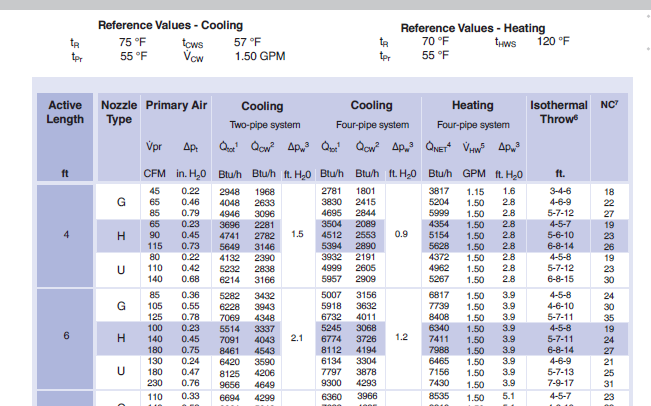
\includegraphics{media/TroxDID632A_Tabledata.png}
\caption{FourPipeBeam/tableData}
\end{figure}

Snippet of catalog data for capacity and primary air flow rate dependence (Trox DID632A)

Choosing a 6 foot beam (with Nozzle type H) at 140 CFM as the rating point, we get 3726 Btu/h = 1092 W, 6 ft = 1.83 m, and 1092/1.83 = 597 W/m for normalized beam cooling capacity at rating point. The associated primary air flow rate of 140 ft\(^{3}\)/min = 0.066 m\(^{3}\)/s and 0.066/1.83 = 0.036 m\(^{2}\)/s is the normalized beam primary air flow rate at the rating point. Note that because the flow rate is normalized by beam length, the units are m\(^{3}\)/s/m (which reduces to m\(^{2}\)/s). The rating heating capacity is listed as a ``net'' heating rate but since this is not well defined in the catalog we go ahead and assume that this represents the beam heating rate where the associated cooling provided by the primary air has already been subtracted. The net heating capacity is 7411 Btu/h = 2172 W. This value need to be increased by the primary cooling provided by 55\(^{\circ}\)F = 12.7\(^{\circ}\)C air entering a zone at 70\(^{\circ}\)F = 21\(^{\circ}\)C. The catalog does not completely define the moist air state of the zone nor the primary air so we assume nominal average moist air density of 1.2 kg/m\(^{3}\) and a specific heat of 1000.0 J/kg-K so that the primary air cooling rate is (21 -- 12.7) * 0.066 * 1.2 * 1000 = 660 W. The beam heating rate is therefore 2172 + 660 = 2832 W. Then normalizing for beam length 2832/1.83 = 1548 W/m is the rated beam heating capacity.

The catalog includes two more data points for capacity at different flow rates, one for 100 ft\(^{3}\)/min and the other for 180 ft\(^{3}\)/min. These are processed in the same way as the rating point data and used to create the modification curves that describe performance as a function of primary air flow rate.

\subsection{Cooled Beam Unit (AirTerminal:SingleDuct:ConstantVolume:CooledBeam)}\label{cooled-beam-unit-airterminalsingleductconstantvolumecooledbeam}

Cooled beam (frequently called chilled beams) systems are usually hybrid water -- air systems. Commonly there is a constant flow, fixed temperature central forced air system for meeting ventilation and latent load requirements.~ Sometimes this forced air system's flow rate is varied according to ventilation demand; and of course its supply air temperature could be reset in various ways. Sensible cooling load is met by the cooled beam units; these are ceiling suspended units with cool water circulating through them. Some types of units are ``passive'' -- they cool by radiation and natural convection. Other types of units are ``active'' and act as supply air terminal units with the supply air inducing room air over the beam cooling elements. These units cool almost entirely by convection. The DOE-2 model (upon which this model is based) is a convection only model -- even the ``passive'' units are assumed to operate 100\% convectively. The cooled beam elements act as an alternative to normal ceiling radiant cooling: they are not coupled to the building mass and they operate more in a convective mode, but they can, like radiant cooling, use fairly warm cooling water.

Heating is accomplished separately from the cooled beam system -- usually baseboards are used on the building perimeter to meet heating loads.

\subsubsection{Model}\label{model-3}

The chilled beam system is modeled as an EnergyPlus terminal unit. In terms of configuration within the overall HVAC system, it resembles a 4 pipe induction terminal unit. The user describes the system as a typical single duct constant volume system (with outside air mixer, fan, heating and cooling coils) on the air loop side, and with cooled beam terminal units on the zone equipment side.

The model is an empirical model developed at the equipment manufacturer Halton Oy. It consists of the following relationships.

The beam cooling output per unit length in W/m is:

\begin{equation}
P_{beam} = A·K·\Delta T
\end{equation}

The coil heat transfer coefficient in W/(m\(^{2}\)K) is:

\begin{equation}
K = \alpha·\Delta T^{n1}·v_{\rho}^{n2}·\omega^{n3}
\end{equation}

The room air mass flow rate across coil in kg/(m\(^{2}\)s) is:
\begin{equation}
v_{\rho} = (q_{in} / \alpha_{0})·\rho_{air}
\end{equation}

The room air volumetric flow rate across coil per unit length in m\(^{3}\)/(s-m) is:

\begin{equation}
q_{in} = K_{1}·\Delta T^{n} + K_{in}·q_{pr}
\end{equation}
 
where:
 
\(\Delta\)T is the room air--water temperature difference (average water temperature is used) in \(^{\circ}\)C

\(\omega\) is the water velocity in m/s

q\(_{pr}\) is the supply air flow rate per unit length m\(^{3}\)/(s-m).

The other symbols are the model parameters input by the user (see the IO Ref for descriptions).

\subsubsection{Inputs and Data}\label{inputs-and-data-3}

The user describes the unit by inputting the name, referencing an availability schedule, and choosing a type (\emph{active} or \emph{passive}). The user must also specify the connectivity of the component by naming the inlet and outlet air and water nodes. The maximum water and fixed air flow rates need to be specified (although these can be autosized). The design inlet and outlet water temperatures are inputs. Generally the inlet water temperature is quite warm (15\(^{\circ}\)C is the default) and the temperature rise is small (design outlet water temperature defaults to 17\(^{\circ}\)C). Two key inputs are the number of beams (in the zone) and the beam length. It is generally wise to let these inputs autosize.

The remaining inputs are parameters specific to the product model. Good defaults are supplied and they should not be changed without information from the manufacturer.

\subsubsection{Sizing}\label{sizing}

The Cooled Beam sizing calculations generally follow the procedures used for other terminal units (see \emph{Loop Equipment Sizing}). One difference is that the Cooled Beams use the Cooled Beam inputs \emph{Design Inlet Water Temperature} and \emph{Design Outlet Water Temperature} for the chilled water \(\Delta\)T rather than the \(\Delta\)T from Plant Sizing. There are also two inputs unique to the Cooled Beam units that are autosized and will be described here.

The input \emph{Number of individual beam units in the zone} is autosized by dividing the beam system zone design chilled water flow rate (either input by the user or autosized) by a nominal chilled water beam flow rate: 0.07 kg/s.

The input \emph{Length of an individual beam unit} is autosized by using the model equations to calculate the length. The inputs to the equations are:

\begin{enumerate}
\item The design load per beam. The design load is calculated from the design water mass flow rate and the design water inlet and outlet temperatures. The design load is divided by the number of beams to obtain the design load per beam.
\item The design air supply air flow per beam -- obtained by dividing the design supply air flow by the number of beams.
\item The design water flow per beam (m\(^{3}\)/s) -- obtained by dividing the design water flow by the number of beams.
\item The design water velocity -- obtained by dividing the design water flow per beam by the cross sectional inside area of a water tube (\(\pi\)D\(^{2}\)/4, where D is the input \emph{Pipe inside diameter}.
\item Average air to water \emph{\(\Delta\)T = T\(_{z,\, cool\, peak}\)} - \emph{0.5(T\(_{w,des\, inlet}\)} \emph{+ T\(_{w,des\, outlet}\))}; where \emph{T\(_{z,\, cool\, peak}\)} is the zone air temperature at the cooling peak and the \emph{T\(_{w,des}\)}'s are the water design inlet and outlet temperatures.
\end{enumerate}

With these inputs the model equations can be solve directly for beam length for passive cooled beams, and iteratively for active cooled beams.

\subsubsection{Calculation}\label{calculation-3}

The subroutine \emph{CalcCoolBeam} uses the model equations to calculate the cooling power \emph{P\(_{beams,out}\)} delivered to the room air and the outlet water temperature given the water flow rate (and the room air temperature and water inlet temperature). Since the model equations are nonlinear they must be solved iteratively. The subroutine does this by varying the outlet water temperature \emph{T\(_{w,out}\)} and calculating the water-side cooling power:

\begin{equation}
P_{w} = q_{w,beam}·c_{p,w}·(T_{w,out}-T_{w,in})
\end{equation}

and comparing it to the air-side cooling power:

\begin{equation}
P_{air} = K·A·\Delta T·L_{beam}
\end{equation}

where \emph{q\(_{w,beam}\)} is the water mass flow rate (kg/s) per beam and \emph{L\(_{beam}\)} is the length of a beam (m). When \emph{P}\(_{w}\) ~and \emph{P\(_{air}\)} match to within 0.1 W the subroutine terminates the iteration.

\subsubsection{Simulation and Control}\label{simulation-and-control-4}

From the result of the zone simulation we have the heating/cooling demand for the zone equipment. For the cooling demand, we use the load to cooling set point \emph{P\(_{c}\)}. Part of the demand may be satisfied by the zone supply air:

\begin{equation}
P_{sup} = q_{air}·(c_{p,air,sys}·T_{sys} - c_{p,air,z}·T_{z})
\end{equation}

The demand on the actual beams is then:

\begin{equation}
P_{beams,dem} = P_{c} - P_{sup}
\end{equation}

We want to know the chilled water flow rate that will give a beam cooling output of \emph{P\(_{beams}\)}. To obtain this we need to numerically invert \emph{CalcCoolBeam}: given its desired output, we want to know the chilled water flow rate. This numerical inversion is carried out by calling the subroutine \emph{SolveRegulaFalsi}. This is a general utility routine for finding the zero of a function (the \emph{residual} function) of a single independent variable. In this case the residual function is basically:

\begin{equation}
(P_{beams,out}-P_{beams,dem})/P_{beams,out,max}
\end{equation}

\emph{SolveRegulaFalsi} varies the cold water mass flow rate to zero the residual. The water inlet and outlet node flow rates are set to the flow rate found by \emph{SolveRegulaFalsi} and the water outlet node temperature is set to the outlet water temperature from \emph{SolveRegulaFalsi}.

\subsubsection{References}\label{references-4}

Documentation Package Update \#2 for DOE-2.1E, Version 107, page 3.152 describes the input and the model for the DOE-2 cooled beam model.

\subsection{Constant Volume Dual Duct Air Terminal}\label{constant-volume-dual-duct-air-terminal}

\subsubsection{Overview}\label{overview-3-000}

The input object AirTerminal:DualDuct:ConstantVolume provides a model for dual duct constant-air-volume (DDCAV) systems that are typically used in special applications where precise temperature and humidity control are required and energy efficiency is not of primary concern. Thermal control for each zone is achieved by mixing air from the hot deck with air from the cold deck to achieve a supply air temperature that will exactly meet the zone load and satisfy the zone thermostat demand. Each zone has its own mixing box which is connected directly to the hot and cold decks. The mixing box dampers change the relative amount of hot and cold air that will be delivered (at a constant volumetric flow rate) to the zone.

\subsubsection{Model Description}\label{model-description-2-000}

The DDCAV model will attempt to meet all of the thermostatic loads of a particular zone by explicitly calculating the hot and cold deck mass flow rates. For the energy and mass balance equations shown below, the zone load, temperatures, specific heats and the design mass flow rate are all known. These equations can then be solved directly for the hot deck and cold deck mass flow rates.

\begin{equation}
\dot Q_{zone} = \dot m_c C_{p,c} T_c + \dot m_h C_{p,h}T_h - \dot m_d C_{p,z} T_z
\end{equation}

\begin{equation}
\dot m_d = \dot m_c + \dot m_h
\end{equation}

where:

\(\dot Q_{zone}\) is the zone load, W (positive = heating, negative = cooling)

\(C_{p,zz}\) is the specific heat of zone air, J/kg-K

\(C_{p,c}\) is the specific heat of cold deck air, J/kg-K

\(C_{p,h}\) is the specific heat of hot deck air, J/kg-K

\({T_z}\) is the zone air dry-bulb temperature, °C

\({T_c}\) is the cold deck air dry-bulb temperature, °C

\({T_h}\) is the hot deck air dry-bulb temperature, °C

\({\dot m_d}\) is the system design air mass flow rate through both heating or cooling duct, kg/s

\({\dot m_c}\) is the cold deck air mass flow rate, kg/s

\({\dot m_h}\) is the hot deck air mass flow rate, kg/s.

\subsubsection{Simulation and Control}\label{simulation-and-control-5}

The simulation first calculates the hot deck and cold deck air mass flow rates required to satisfy the heating/cooling demand on the zone. Once the individual flow rates have been calculated based on temperature control, the zone mixed air conditions are calculated assuming adiabatic mixing of the two air streams.

\subsection{Variable Air Volume Dual Duct Air Terminal}\label{variable-air-volume-dual-duct-air-terminal}

\subsubsection{Overview}\label{overview-4-000}

The input object AirTerminal:DualDuct:VAV provides a model for dual duct variable-air-volume (DDVAV) systems that are typically used in special applications where both temperature and humidity control as well as energy efficiency are of primary concern.~ This system combines the advantages of the standard dual duct system for better thermal control with the possibility to reduce fan energy using a variable speed fan. The DDVAV terminal units contain actuated dampers that vary the amount of central system air supplied to a zone from both the hot and cold deck. Optional user inputs may also be used to control the amount of outdoor air entering the zone.

The DDVAV terminal units described here are used primarily with central air handling equipment with cooling and heating capability. The terminal unit dampers modulate the amount of cold air and hot air as well as the overall flow rate to maintain the zone setpoint temperature(s).

\subsubsection{Model Description}\label{model-description-3-000}

The DDVAV model will attempt to meet all of the thermostatic loads of a particular zone by first sending air through either the heating duct or the cooling duct depending on whether there is a heating or cooling load (respectively).~ Flow rate through the opposite duct is kept at zero and flow through the active duct is varied between the minimum air flow rate (minimum zone air fraction multiplied by the maximum flow rate) and the maximum air flow rate.~ If the flow rate to meet the load through either the heating or cooling duct results in a flow outside these ranges, then air must be passed through the other duct as well to avoid over- or under-heating or --cooling. This is done using a conservation of energy and mass analysis of the terminal unit as well as the known inlet and necessary outlet condition to meet the thermal needs of the zone.

When there is no load on the zone, the system could either be scheduled off or be in a ``no load'' condition.~ If the system is scheduled off, the model keeps the flow rate at zero for both the heating and cooling duct.~ If in a no load condition, the system attempts to throttle back to the minimum possible flow and then find a balance between flow through the heating and cooling duct that will provide no net conditioning to the space.~ This means that the enthalpy of air delivered to the space must be equal to the enthalpy of the (average) air in the zone.

\subsubsection{DDVAV Terminal Unit Inputs}\label{ddvav-terminal-unit-inputs}

Like other terminal units, the DDVAV terminal unit requires an availability schedule and inlet and outlet node designations.~ The DDVAV terminal unit, like the DD terminal unit, has two inlet nodes (one for the heating duct and one for the cooling duct) and one outlet node.

In addition, the DDVAV terminal unit also has a maximum flow rate and a minimum flow fraction like the VAV terminal unit.~ This allows the flow to be throttled back when it is possible to provide the proper amount of conditioning with less flow.~ The maximum flow rate can be auto-sized, if desired.

\subsubsection{Minimum Outdoor Air Control}\label{minimum-outdoor-air-control-1}

This dual duct air terminal may also be used to provide a minimum outdoor air quantity. When the air flow rate required to meet the zone load does not provide sufficient outdoor air, the terminal device damper will open to allow sufficient outdoor air to enter the zone. In this case, the terminal damper is controlled based on the air loop's outdoor air fraction. The outdoor air may be specified as a fixed value per person, per floor area, or per zone or as the required minimum air changes per hour. In addition, these values may be added together to provide a combined minimum outdoor air flow rate or the maximum of each of these values may be used. An outdoor air fraction schedule may also be used to modify the calculation for the minimum amount of outdoor air throughout the simulation (Ref. DesignSpecification:OutdoorAir).

\subsubsection{Simulation and Control}\label{simulation-and-control-6}

The simulation begins by determining the air mass flow rate required to satisfy the heating/cooling demand using either the heating duct or cooling duct.

\begin{equation}
C_{p,zone} = PsyCpAirFnWTdb\left( {\omega_{zone}},{T_{zone}} \right)
\end{equation}

\begin{equation}
C_{p,inlet} = PsyCpAirFnWTdb\left( {\omega_{inlet}},{T_{inlet}} \right)
\end{equation}

\begin{equation}
\Delta C_p T = \left( {C_{p,inlet}} \right)\left( {{T_{inlet}}} \right) - \left( {C_{p,zone}} \right)\left( {{T_{zone}}} \right)
\end{equation}

\begin{equation}
\dot m = \min \left( \dot m_{max}, \max \left( \dot m_{max}\cdot MinAirFlowFrac,\frac{\dot Q_{zone}}{\Delta C_p T} \right) \right)
\end{equation}

where

\(C_{p,zone}\) is the specific heat of zone air, J/kg-K

\(C_{p,inlet}\) is the specific heat of terminal unit inlet air, J/kg-K

\({\omega_{zone}}\) is the zone air humidity ratio, kg/kg

\({T_{zone}}\) is the zone air dry-bulb temperature, °C

\({\omega_{inlet}}\) is the terminal unit inlet air humidity ratio, kg/kg

\({T_{inlet}}\) is the terminal unit inlet air dry-bulb temperature, °C

\(\dot Q_{zone}\) is the zone load, W (positive values denote heating, negative values denote cooling)

\(\dot m\) is the terminal unit air mass flow rate through either heating or cooling duct, kg/s

\(PsyCpAirFnWTdb\) is the psychrometric function calculating air specific heat given air humidity ratio and dry-bulb temperature

\(MinAirFlowFrac\) is the user-specified zone minimum air flow fraction

\({\dot m_{max}}\) is the terminal unit maximum air mass flow rate, kg/s.

The outdoor air input requirements, if entered, are then used to adjust the terminal unit air mass flow rate to ensure the correct amount of outdoor air enters the zone (within the constraints of the terminal unit maximum and minimum flow rate inputs). The amount of outdoor air is calculated per the outdoor air requirements and is adjusted by the fraction of outdoor air entering the air loop outdoor air system.

\begin{equation}
  \dot{m} = \max\PB{ \dot{m}, \frac{\dot{m}_{OA}}{OAFrac} }
\end{equation}

where:

\(\dot m_{OA}\) is the zone outdoor air flow rate, kg/s

\(OAFrac\) is the fraction of outdoor air entering the air loop outside air system.

The damper position is then calculated as:

\begin{equation}
  FRAC_{damper} = \frac{\dot{m}}{\dot{m}_{max}}
\end{equation}

where \(FRA{C_{damper}}\) is the output variable `Zone Air Terminal VAV Damper Position' in fraction of maximum flow.

If the flow rate was between the maximum flow rate and the minimum flow rate for the terminal unit, then no other calculations are needed.~ However, if the flow was reset to either the maximum or minimum flow rate, then flow through the active duct must be balanced by flow through the other duct to achieve the proper conditioning.

\subsubsection{References}\label{references-5}

No specific references.~ Refer to the ASHRAE Handbook series for general information on different system types as needed.

\subsection{Dual Duct Dedicated Outside Air Terminal with VAV Cooling}\label{dual-duct-dedicated-outside-air-terminal-with-vav-cooling}

\subsubsection{Overview}\label{overview-5-000}

The input object AirTerminal:DualDuct:VAV:OutdoorAir provides a model for dedicated outside air combined with recirculated air for cooling.~ This air terminal has two inlets and one outlet. The outdoor air inlet has one damper that is controlled to meet the air flow requirements for ventilation.~ The second inlet is for cool recirculated air and has a second damper that is controlled to meet the zone's cooling loads.~ The two streams are then mixed and inlet to the zone.~ This unit is for central air systems (using AirLoopHVAC object). ~Because of the limitation in EnergyPlus of allowing only one air terminal per zone, the dual duct approach offers advantages in that it allows modeling dedicated outdoor air systems (DOAS) and central VAV cooling at the same time.~ The original motivation for adding this terminal was to model twin-fan, twin-coil systems.

The recirculated cool air duct is actually optional. If no node name is input for the recirculated air inlet node, then only the outdoor air duct is operational and the air terminal behaves as a single duct.~ This offers additional capabilities for single duct DOAS in that this terminal can request outdoor air flows that change over time but are not controlled to meet zone loads.

\subsubsection{Model Description}\label{model-description-4-000}

The model attempts to meet the ventilation requirements and the cooling loads of a particular zone.~ If the zone requires heating, ancillary heating equipment is needed as this terminal cannot do any heating.~ The model first determines the current required outdoor air flow rate for ventilation and then calculates the flow of cool air needed to reach the cooling setpoint.

The outdoor air rate is controlled by the schedule and specifications contained in a DesignSpecification:OutdoorAir object and can be based on flows per person, per zone, per area, or air changes per hour.~ Using the key CurrentOccupancy, the per person rate can be set to operate based on the current occupancy level to model demand controlled ventilation. Using the key DesignOccupancy it can be set to operate based on the design, or maximum, level of occupancy.~~ The outdoor air inlet side of the terminal is assigned a design maximum flow rate based on the largest flow rates specified by the associated DesignSpecification:OutdoorAir object. This maximum for the outdoor air is used to calculate the damper position and contributes to the overall maximum if that is autosized.

The recirculated cool air flow rate is controlled to meet the zone cooling loads.~ The first step is to calculate the impact that the outdoor air flow has on the loads starting with the specific heats.

\begin{equation}
{c_{p,zone}} = PsyCpAirFnWTdb\left( {{\omega_{zone}},{T_{zone}}} \right)
\end{equation}

\begin{equation}
{c_{p,OA}} = PsyCpAirFnWTdb\left( {{\omega_{OA}},{T_{OA}}} \right)
\end{equation}

\begin{equation}
{c_{p,RC}} = PsyCpAirFnWTdb\left( {{\omega_{RC}},{T_{RC}}} \right)
\end{equation}

where:

\(c_{p,zone}\) is the specific heat of zone air being served by the terminal unit, J/kg-K

\(c_{p,OA}\) is the specific heat of outdoor air entering the terminal unit, J/kg-K

\(c_{p,RC}\) is the specific heat of the recirculated (cool) air entering the terminal unit (if present), J/kg-K

\(\omega_{zone}\) is the humidity ratio of the zone air, kg/kg

\(\omega_{OA}\) is the humidity ratio of the outdoor air entering the terminal unit, kg/kg

\(\omega_{RC}\) is the humidity ratio of the recirculated air entering the terminal unit, kg/kg

\(T_{zone}\) is the air drybulb temperature of the zone, \(^{\circ}\)C

\(T_{OA}\) is the air drybulb temperature of the outdoor air entering the terminal unit, \(^{\circ}\)C

\(T_{RC}\) is the air drybulb temperature of the recirculated cool air entering the terminal unit, \(^{\circ}\)C

\(PsyCpAirFnWTdb\) is a psychrometric function for calculating the specific heat of moist air as a function of humidity ratio and drybulb temperature.

The contribution to zone load provided by the outdoor air toward meeting the cooling setpoint, \({\dot Q_{OA}}\) (W), is then calculated using:

\begin{equation}
{\dot Q_{OA}} = {\dot m_{OA}}\left( {{c_{p,OA}}{T_{OA}} - {c_{p,zone}}{T_{zonesetpoint}}} \right)
\end{equation}

where:

\(\dot{m}_{OA}\) is the mass flow rate of outdoor air determined by the outdoor air requirement, kg/s

\(T_{zonesetpoint}\) is the zone cooling setpoint drybulb temperature, \(^{\circ}\)C.

This is then used to calculate the load that the recirculated cool air should deliver, \({Q_{RC}}\) (W):

\begin{equation}
{\dot Q_{RC}} = {\dot Q_{ToCoolSetpointRemain - }}{\dot Q_{OA}}
\end{equation}

where \({\dot Q_{ToCoolSetpointRemain = }}\) is the remaining load to cooling setpoint as determined by Predictor and including the impacts of any other zone equipment sequenced before this terminal. Then the recirculated cool air mass flow rate, \({\dot m_{RC}}\) (kg/s), is calculated using:

\begin{equation}
{\dot m_{RC}} = \frac{{{{\dot Q}_{RC}}}}{{\left( {{c_{p,RC}}{T_{RC}} - {c_{p,zone}}{T_{zone}}} \right)}}
\end{equation}

The model also includes a form of damping where the last three values for \({\dot m_{RC}}\) are stored and used to detect if the solution is oscillating from one iteration to the next and if it is then the new value is not used but rather the value from the previous iteration is used.~ Once the two mass flows are known, the moist air properties of the outlet node are calculated using mass flow weighting.

\subsubsection{References}\label{references-6}

Sekhar, S. C., K. W. Tham, et al. (2004). Development of energy-efficient single-coil twin-fan air-conditioning system with zonal ventilation control, Nashville, TX, United states, Amer. Soc. Heating, Ref. Air-Conditoning Eng. Inc.
